\documentclass[a4paper,12pt]{article}
\usepackage[utf8x]{inputenc}
\usepackage[T1]{fontenc}
\usepackage[french]{babel}
\usepackage{graphicx}
\graphicspath{ {images/} }
\usepackage{float}
\usepackage{listings}
\usepackage{color}

\setlength{\parindent}{0cm}
\setlength{\parskip}{1ex plus 0.5ex minus 0.2ex}

\title{Organisation de travail}
\author{Mohammad Nauval}

\begin{document}
\maketitle

Dans cette partie, nous examinons l'organisation de notre projet de compilation. Ce projet développé par une équipe de six personnes, est pour nous l'occasion d'expérimenter le développement en agilité, évoqué en cours de génie logiciel. L'agilité est une approche basée sur 12 principes et 4 valeurs\footnote{http://agilemanifesto.org/iso/fr/principles.html}. Le développement agile est entre autres basé sur la collaboration entre le client du produit et les développeurs. Il prévoit de satisfaire le besoin client en livrant des versions fonctionnelles du produit, de manière itérative et incrémentale. 

L'un de principe d'agilité dit de "livrez fréquemment un logiciel opérationnel avec des
cycles de quelques semaines à quelques mois et une préférence pour les plus courts". Alors le développement du logiciel en agilité progressent par des sprints. Dans chaque sprint développement du logiciel fait un cycle. Ce la veut dire que les fonctionnalités sont conçues, codées et testées. Le logiciel est livré régulièrement aux clients dans chaque release, qui consiste à quelques sprints. 

Alors nous avons décider d'effectuer 2 livraisons et chaque release composé de 3 sprints de 2 semaines.   

\section{Outils}
\subsubsection{Trello}
\textcolor{red}{Dire c'est quoi trello}

\subsubsection{Slack}
\textcolor{red}{Dire c'est quoi slack et pourquoi on a utilisé}

\section{Organisation de travail}
\subsection{Produit finale et ses versions}
Avant le développement, nous avons défini des fonctionnalités que notre projet doit accomplir. Les exigences sont exprimé en tant que user story et stocké dans le backlog du produit.
Comme mentionné ci-dessus nous livrons le produit en 2 releases : fonctionnalités sont ensuite découpées pour chaque \textit{release}.

\begin{figure}[H]
\begin{center}
	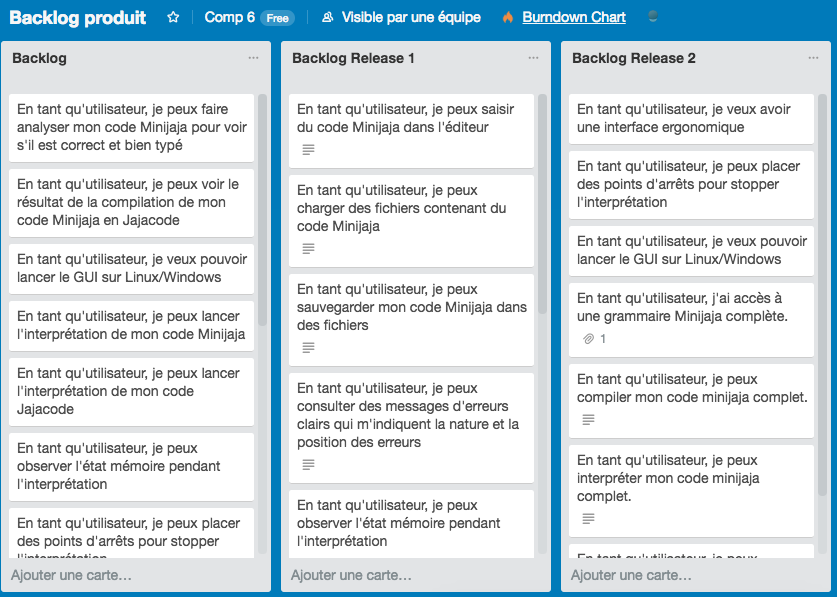
\includegraphics[scale=0.3]{backlogproduit}
	\caption{Backlog produit du projet}
\end{center}
\end{figure}

Car l'agilité s'appuie sur une équipe auto-organisationnelle, nous avons amener de définir les fonctionnalités fournies pour le release 1.  Alors pour release 1 nous avons décider  d'implémenter les fonctionnalités suivantes :

L'utilisateur peut saisir le code source MiniJaja réduite (MiniJaja qui permet avoir des variable de type int et permet d'additionner des nombres ou des variables), vérifier que le code source ne contient pas des erreurs de typages, le compiler ver le JajaCode et l'interpréter. De plus, permettre aux utilisateurs exécuter le JajaCode obtenu. Étant conscient que les clients (les utilisateurs à qui destiné le logiciel), n'ont pas des compétences techniques pour utiliser les fonctionnalités fournie sans interface homme-machine, bien évidement, qu'il y aura une interface utilisateur minimum ergonomique pour faciliter l'utilisation de notre logiciel.
 
Nous avons décider de développer presque toutes les fonctionnalités attendues du produit final (sauf l'exécution pas-à-pas et point d'arrêt) pour une grammaire réduite, car ça nous permet fournir un logiciel fonctionnel pour le premier release et avoir retour de client sur implémentations des exigences.  

Pour le release 2 nous avons prévus que le logiciel va contenir les fonctionnalités attendues pour un produit finale. 

\subsection{Organisation de sprint}
Comme ce que nous avons déjà mentionné, avec l'approche d'agilité, nous organisons le travail en plusieurs cycles appelant sprint. 

Au début de chaque sprint, nous avons organisé une réunion pour définir les tâches que nous avons eu à compléter à la fin du sprint. Pour cela, nous avons examiné le \textit{backlog} de \textit{release} suivant, à partir des fonctionnalités décrites dans ce dernier, nous avons pu extraire les tâches à compléter. Le but c'était de pouvoir implémenter toutes les fonctionnalités décrites dans le backlog de chaque \textit{release} à la fin de trois sprints.

Ensuite, nous avons crée un tableau pour chaque sprint. Dans le tableau, il y a eu trois 4 listes. La première, c'était la liste de tâches à faire. La deuxième et troisième sont la liste de tâches en cours de réalisation et la liste de tâches finies à vérifier. Et la dernière liste, c'était la liste de tâches complétées.

Dans la réunion au début de chaque sprint, chaque membre de l'équipe a choisit les tâches qu'il voulait faire. La réalisation de tâche peut aussi se faire en binôme si sa taille est assez importante. La personne responsable de chaque tâche devait informer son avancement en modifiant l'état de tâche (en cours, à vérifier, ou finie). Pour chaque tâche, nous avons aussi prévu sa durée de réalisation et à la complétion d'une tâche, la durée réelle de ce dernier est aussi révélée.

Par example, voici à ce quoi notre tableau de deuxième sprint de \textit{release} 1 ressemble.

\begin{figure}[H]
\begin{center}
	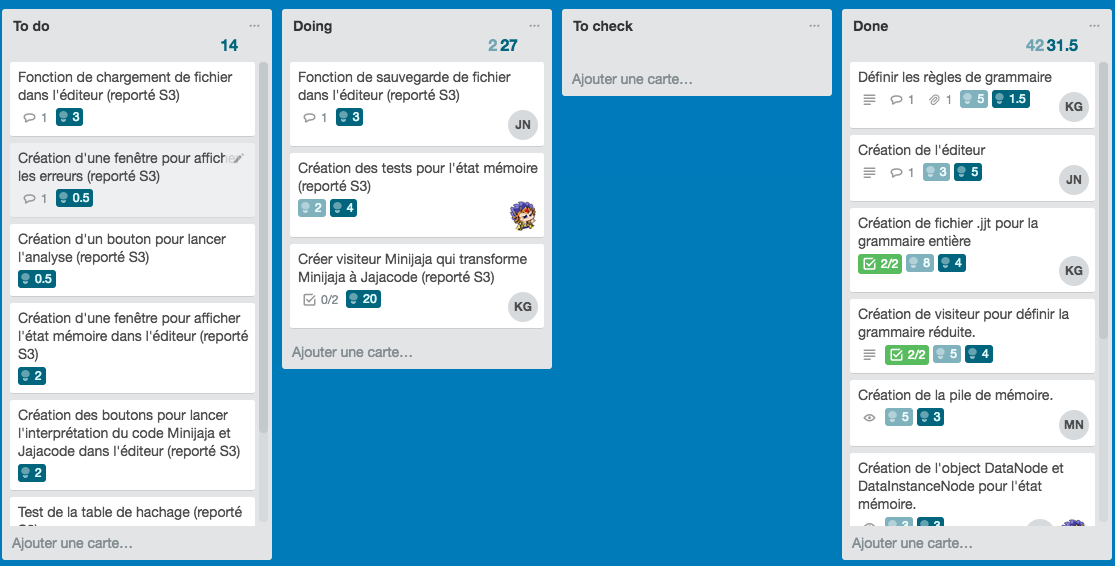
\includegraphics[scale=0.3]{sprint2}
	\caption{Tableau d'organisation de travail de sprint 2 de \textit{release} 1}
\end{center}
\end{figure}

Les tâches non-complétées doivent être reportées au sprint suivant. La personne travaillant sur une tâche doit aussi s'occuper de la réalisation des tests pour vérifier ce qui a été fait.
\section{Réunions}
\subsubsection{Réunions régulière}
\textcolor{red}{pandent tp, entre sprint pour faire point d'avancement, technique}


\subsubsection{Révue de sprint}
\textcolor{red}{Ce qu'on fessait à la fin de chaque sprint}

\subsubsection{Rétrospective}
\textcolor{red}{Dire un eu qu'on a fait retrospective et que plus de détails seront donnés dans la parties rétrospective}

\end{document}